\begin{figure}[tpb]
    \begin{minipage}[h]{0.49\linewidth}
    \center{
        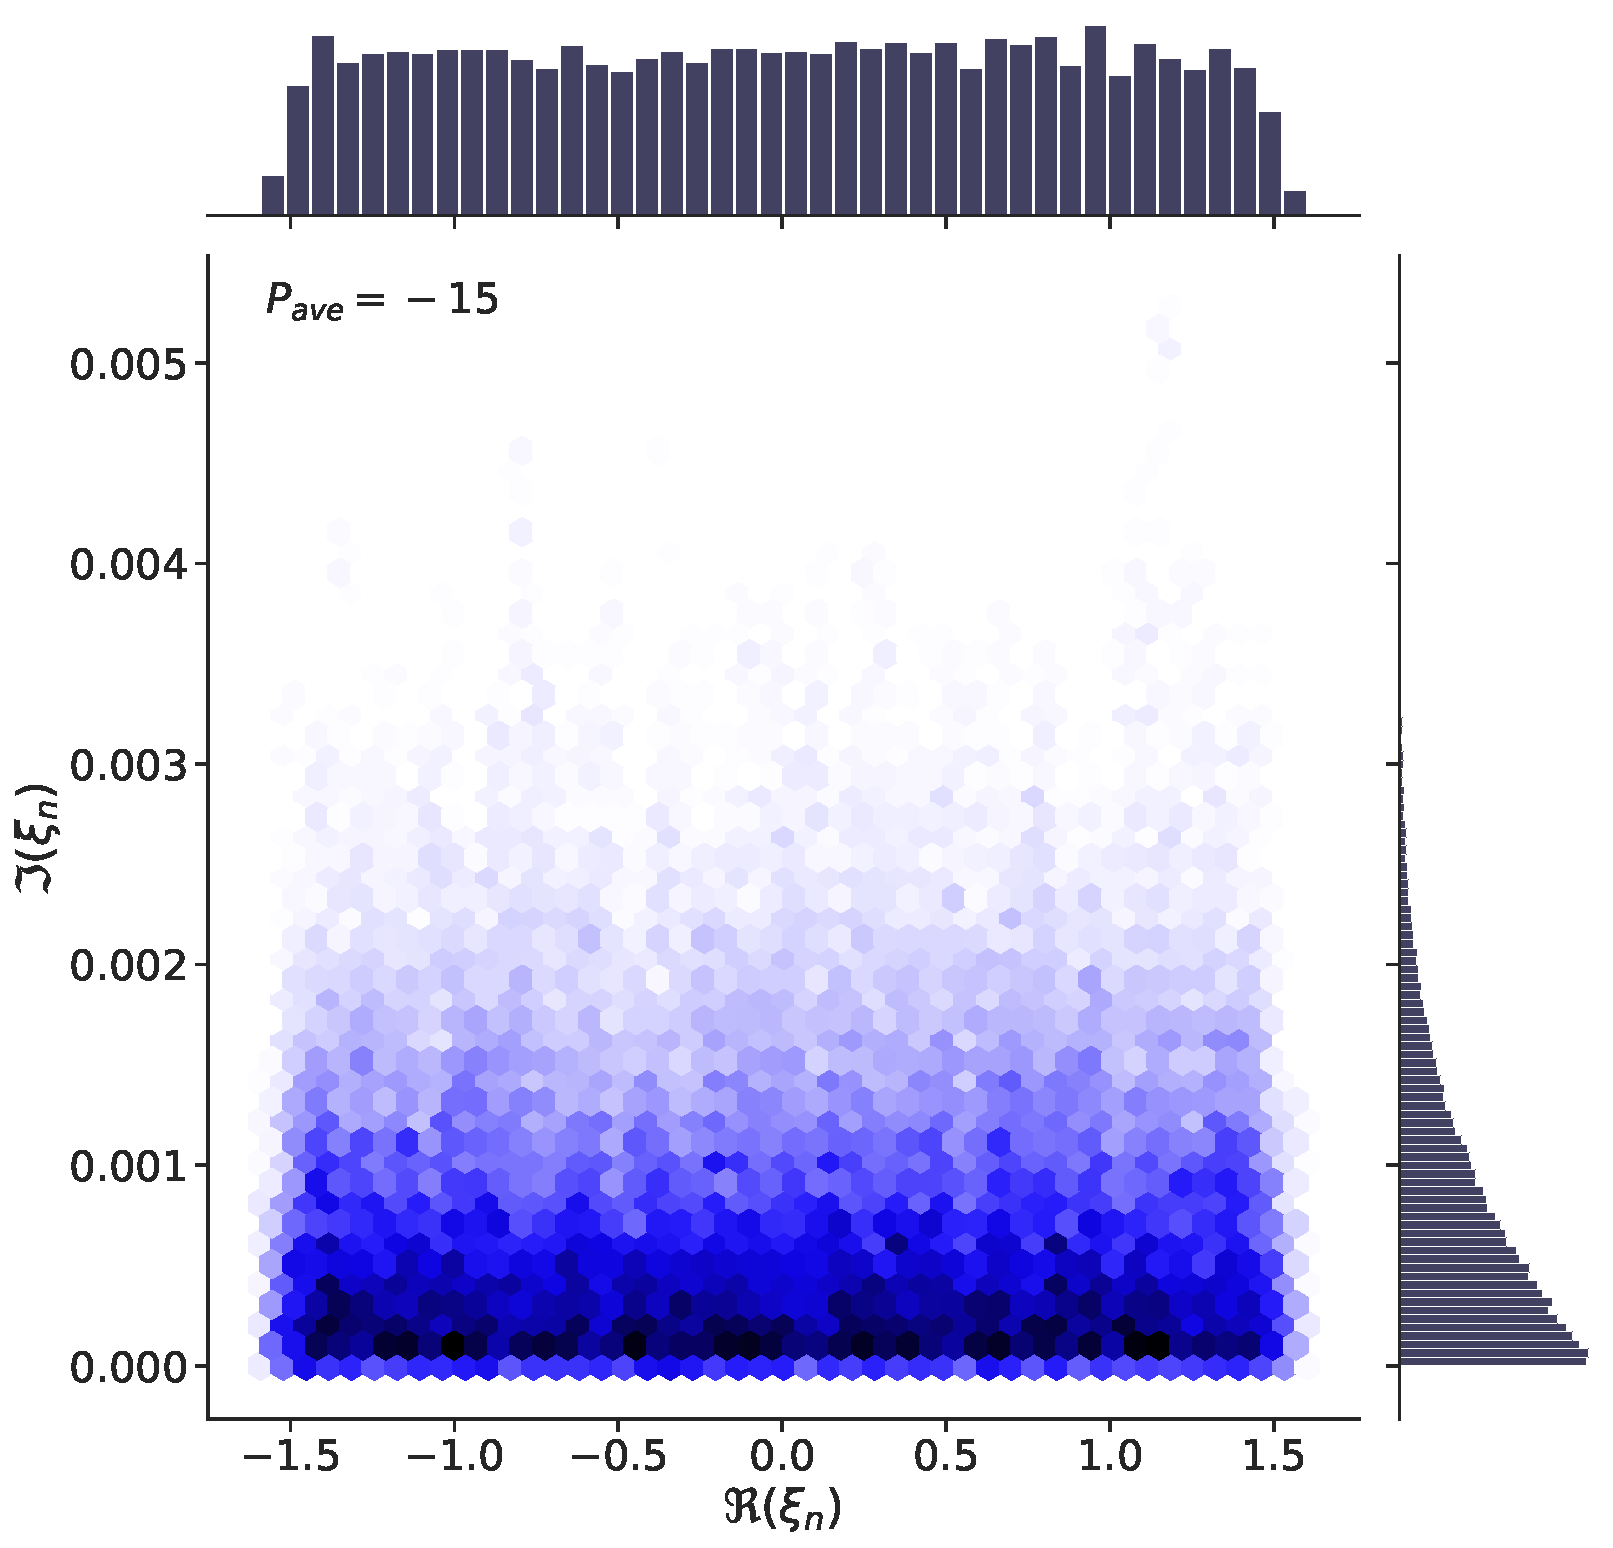
\includegraphics[width=1\linewidth]{images/soliton/wdm_trans/discrete_spectrum_distribution_pavedbm_-15.pdf} \\
    }
    \end{minipage}
    \hfill
    \begin{minipage}[h]{0.49\linewidth}
    \center{
        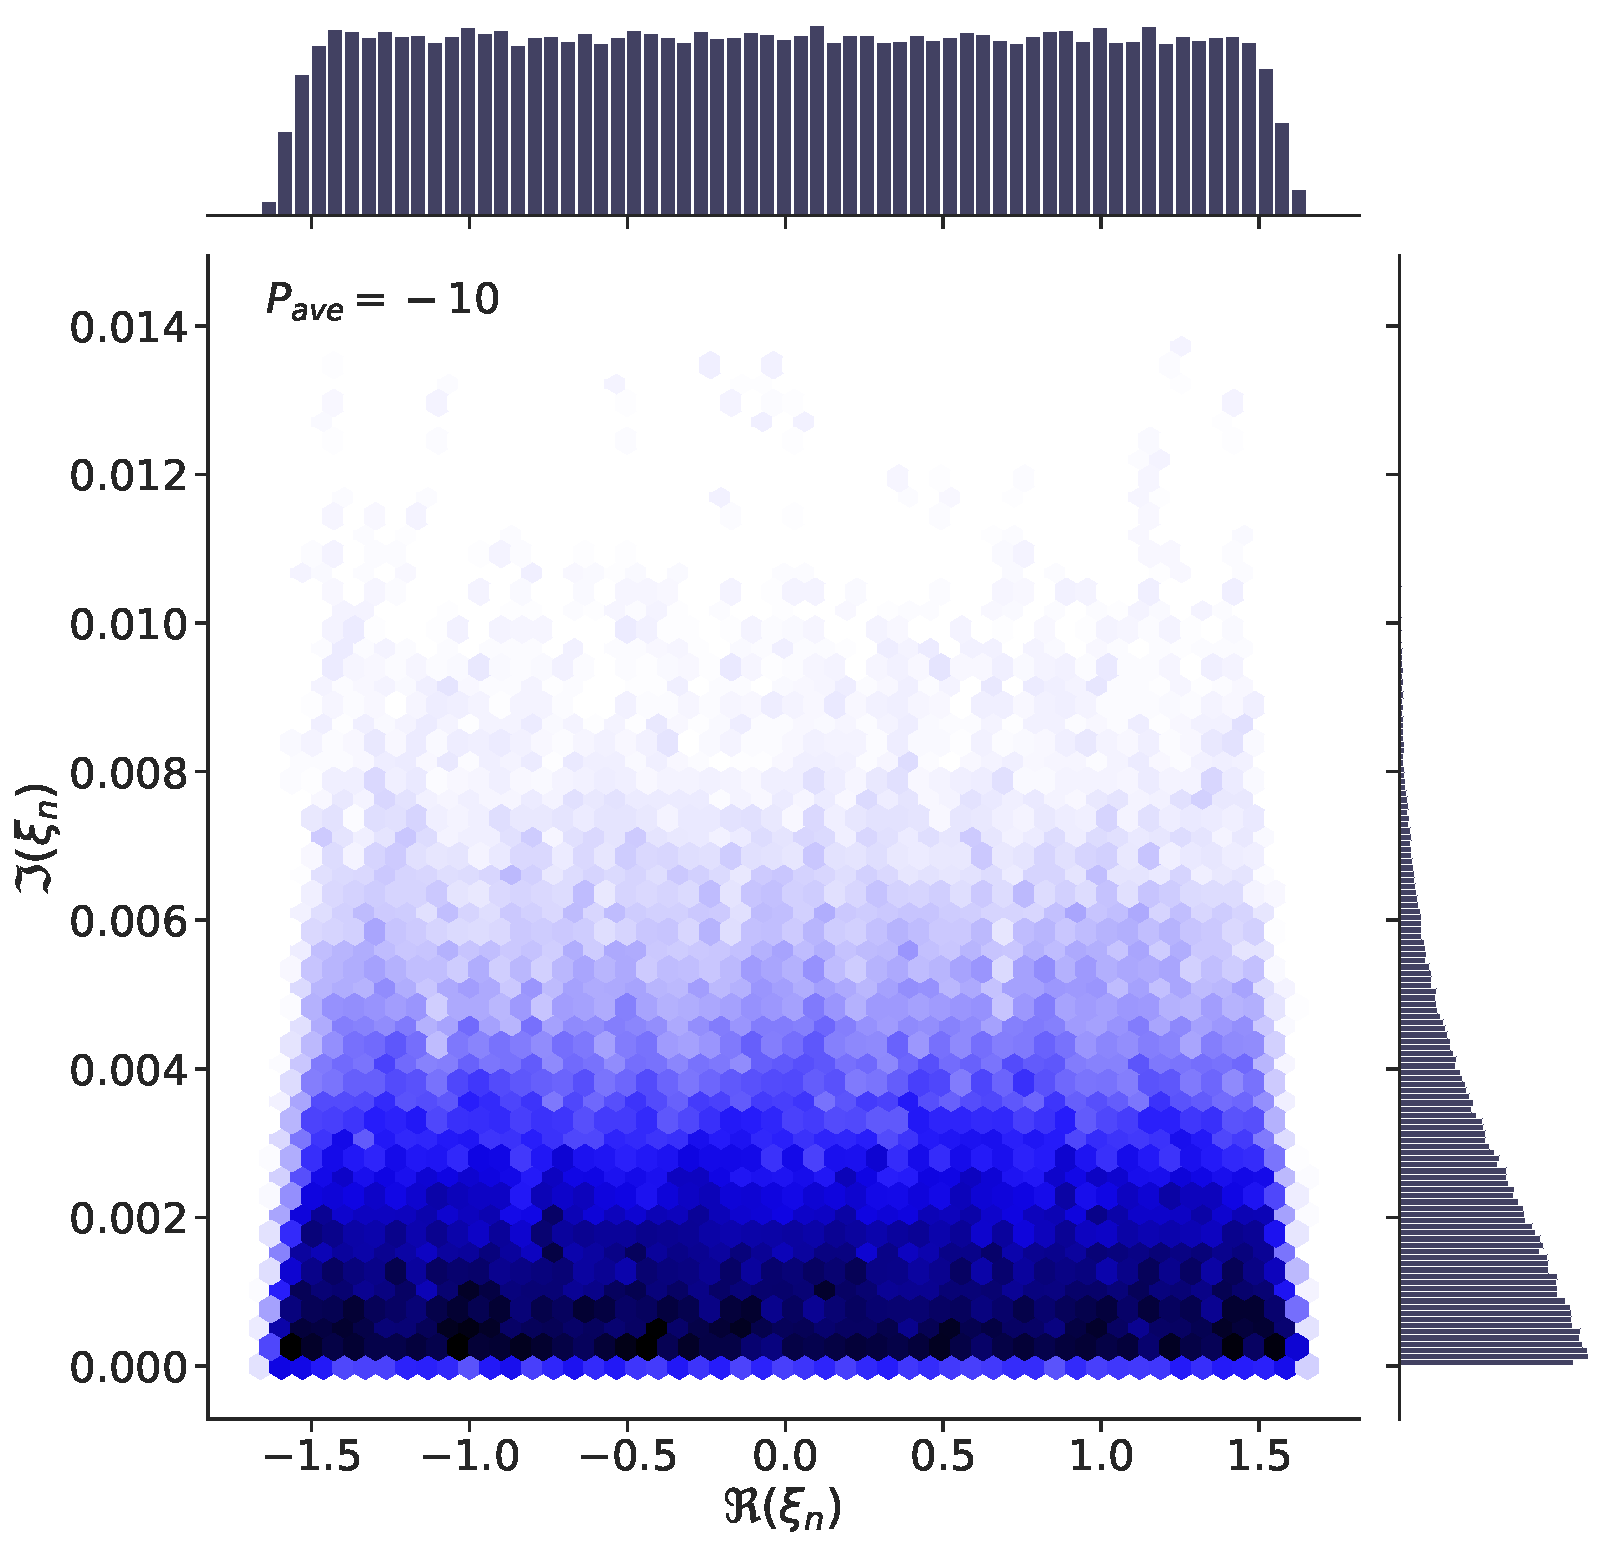
\includegraphics[width=1\linewidth]{images/soliton/wdm_trans/discrete_spectrum_distribution_pavedbm_-10.pdf} \\
    }
    \end{minipage}

    \begin{minipage}[h]{0.49\linewidth}
    \center{
        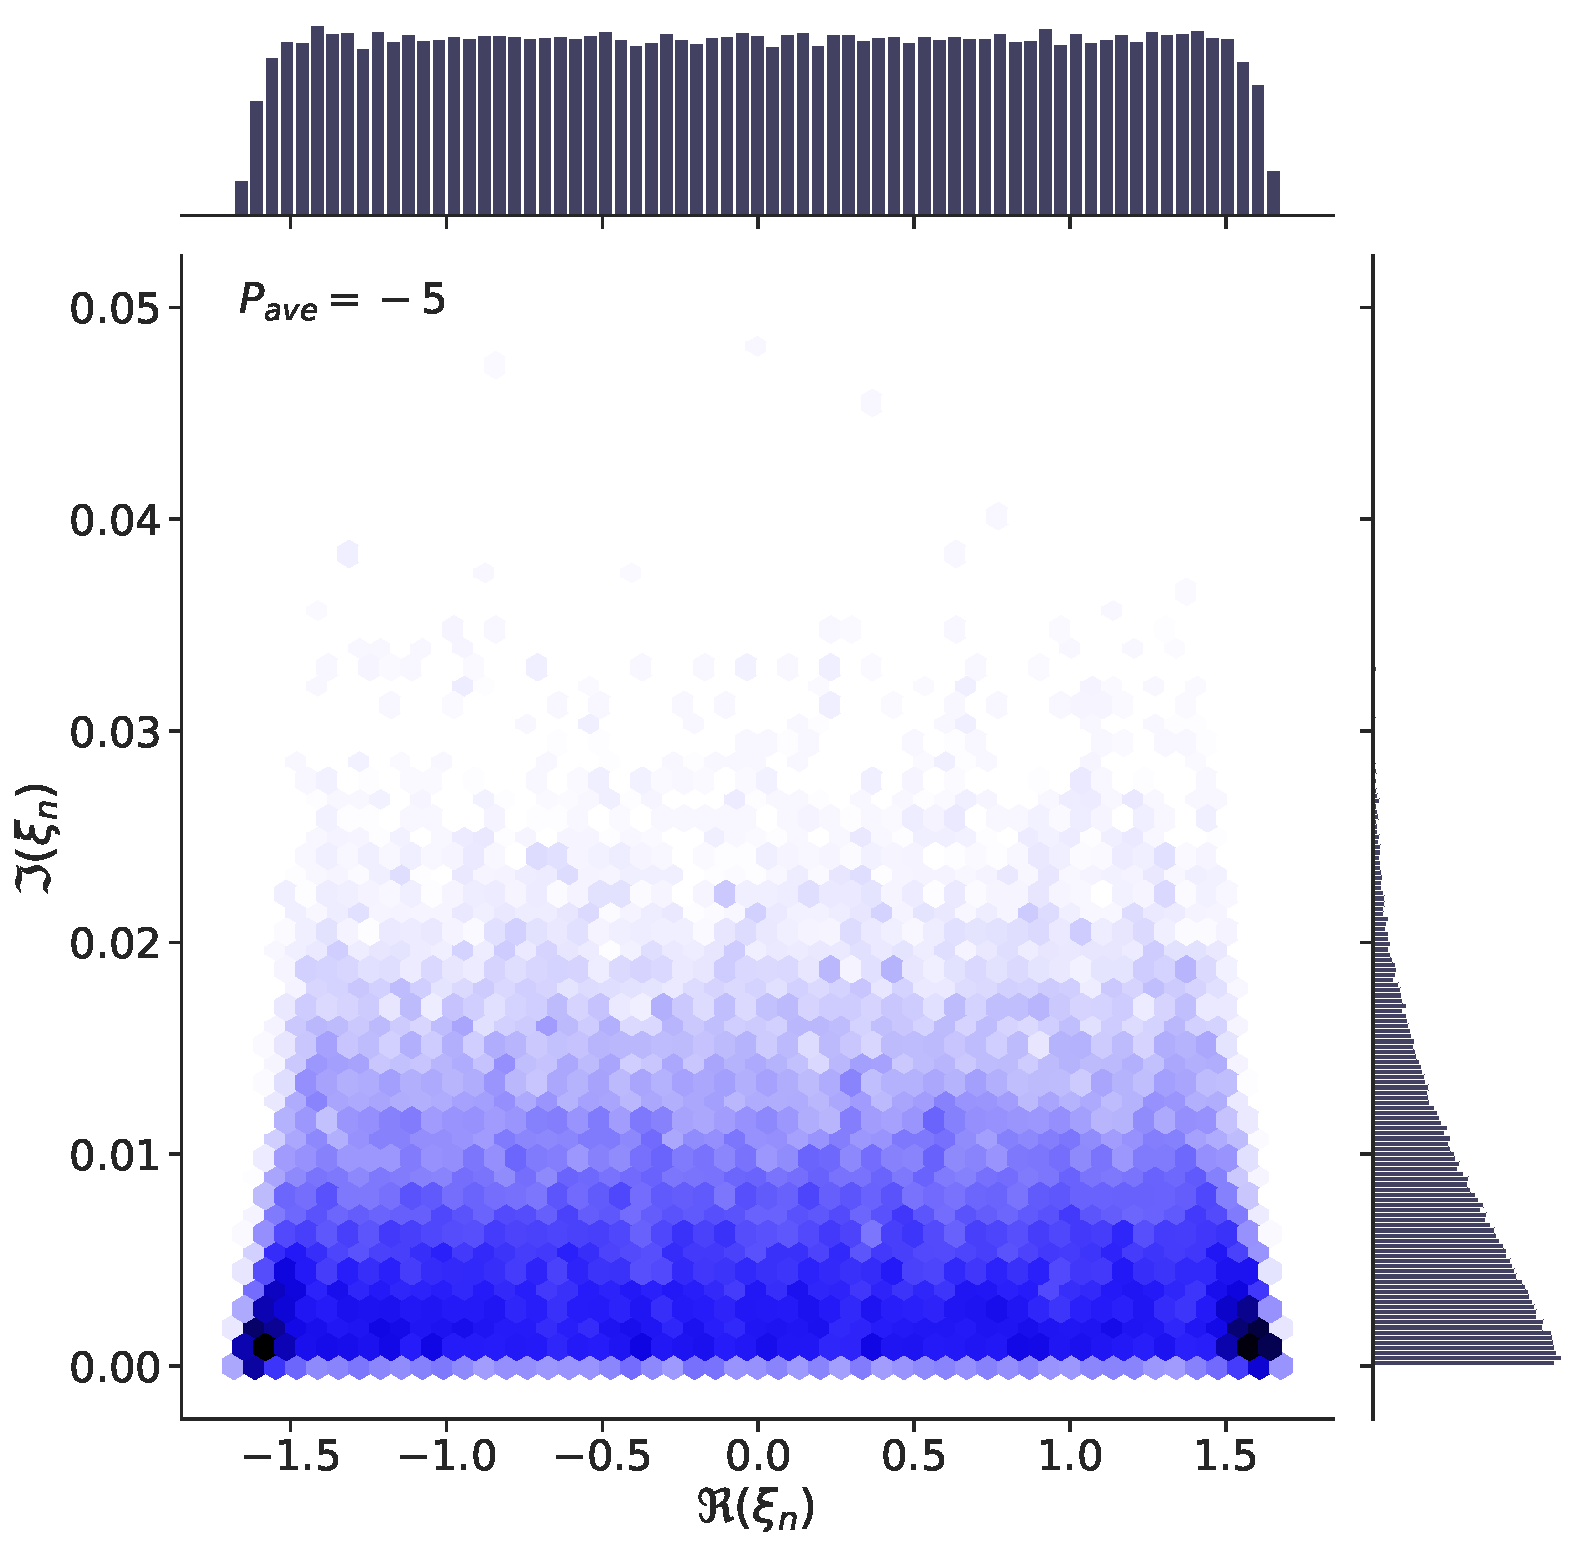
\includegraphics[width=1\linewidth]{images/soliton/wdm_trans/discrete_spectrum_distribution_pavedbm_-5.pdf} \\
    }
    \end{minipage}
    \hfill
    \begin{minipage}[h]{0.49\linewidth}
    \center{
        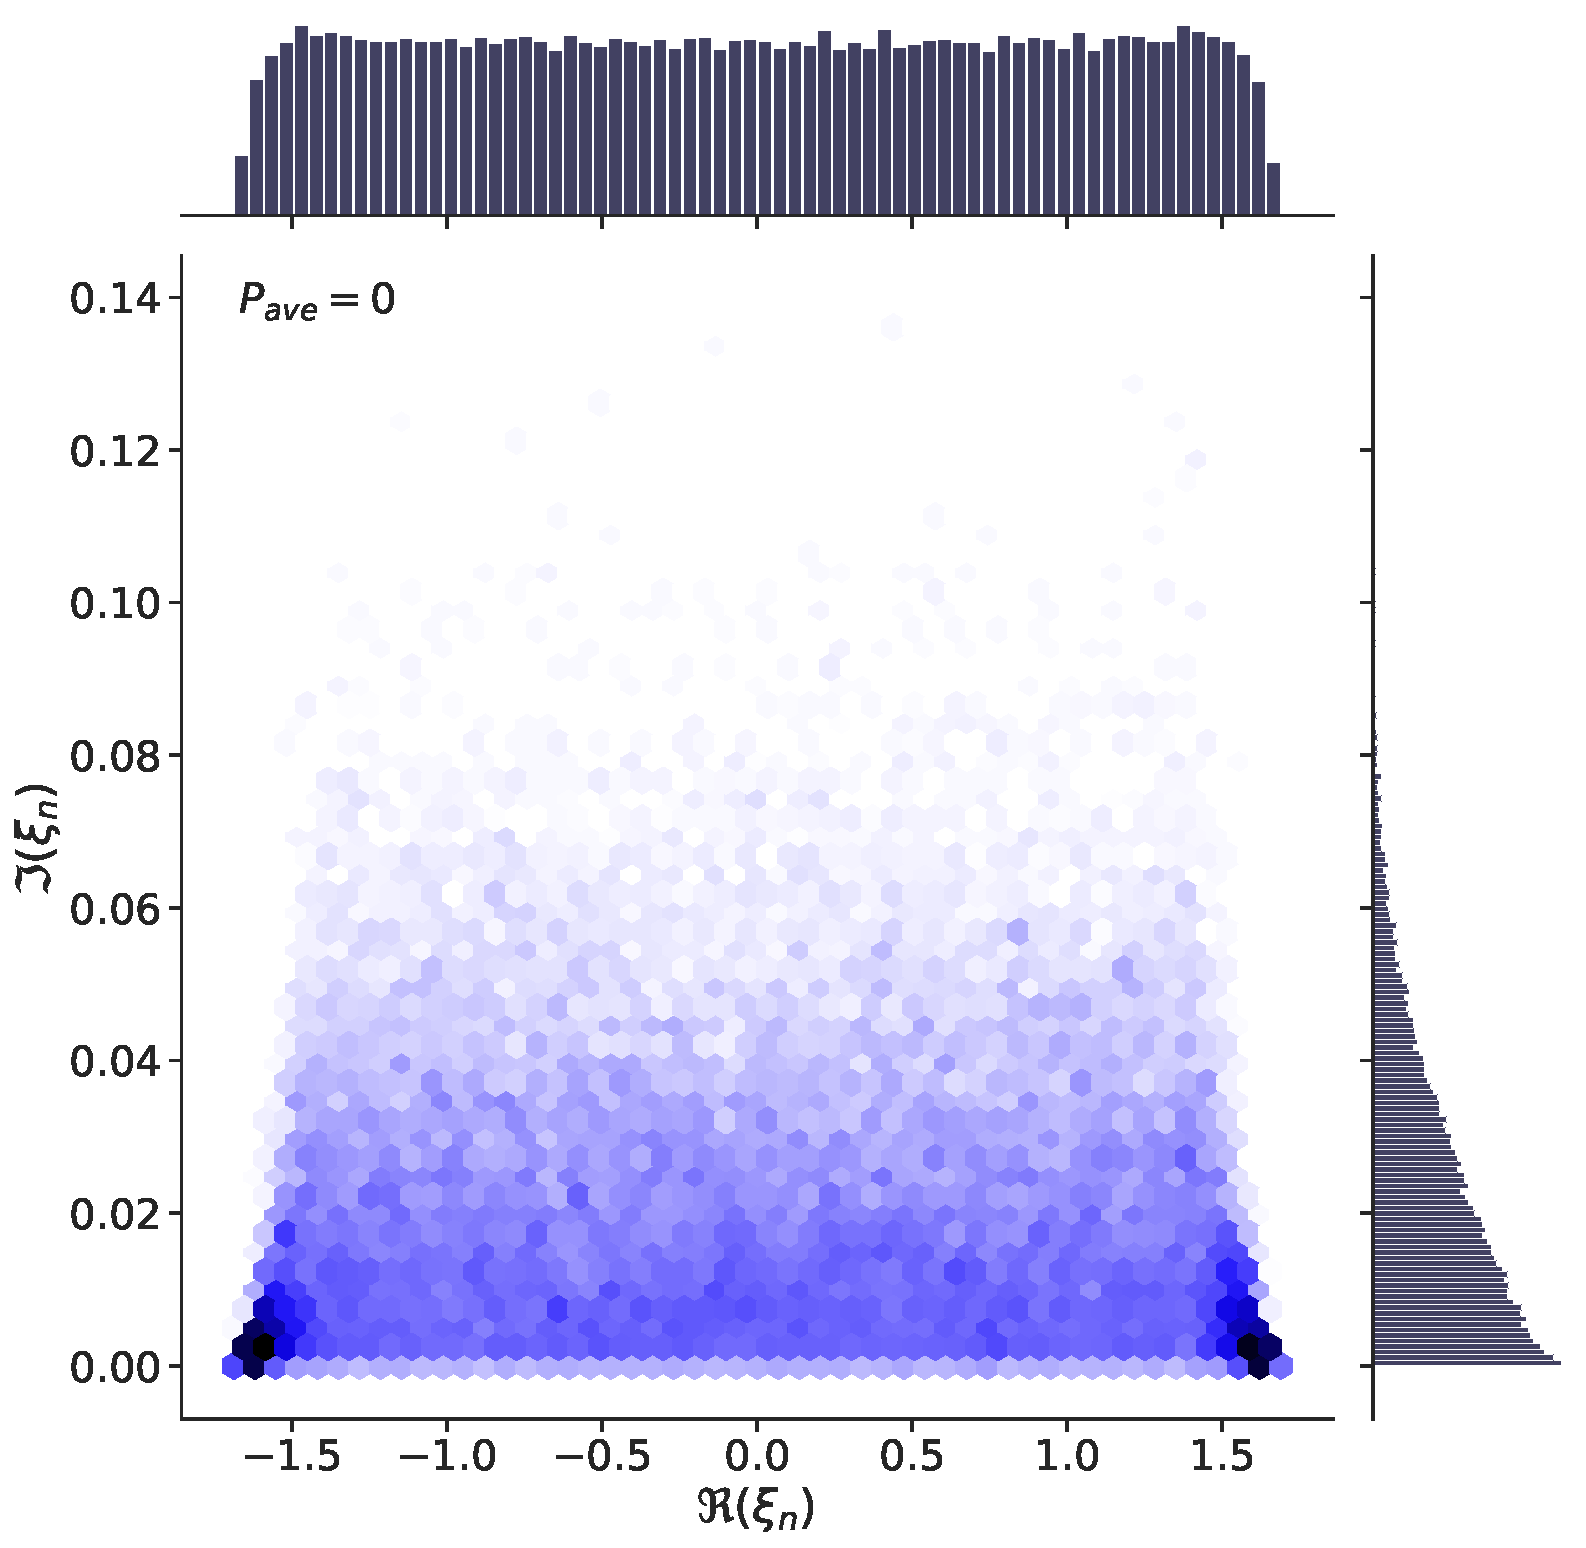
\includegraphics[width=1\linewidth]{images/soliton/wdm_trans/discrete_spectrum_distribution_pavedbm_0.pdf} \\
    }
    \end{minipage}

    \begin{minipage}[h]{0.49\linewidth}
    \center{
        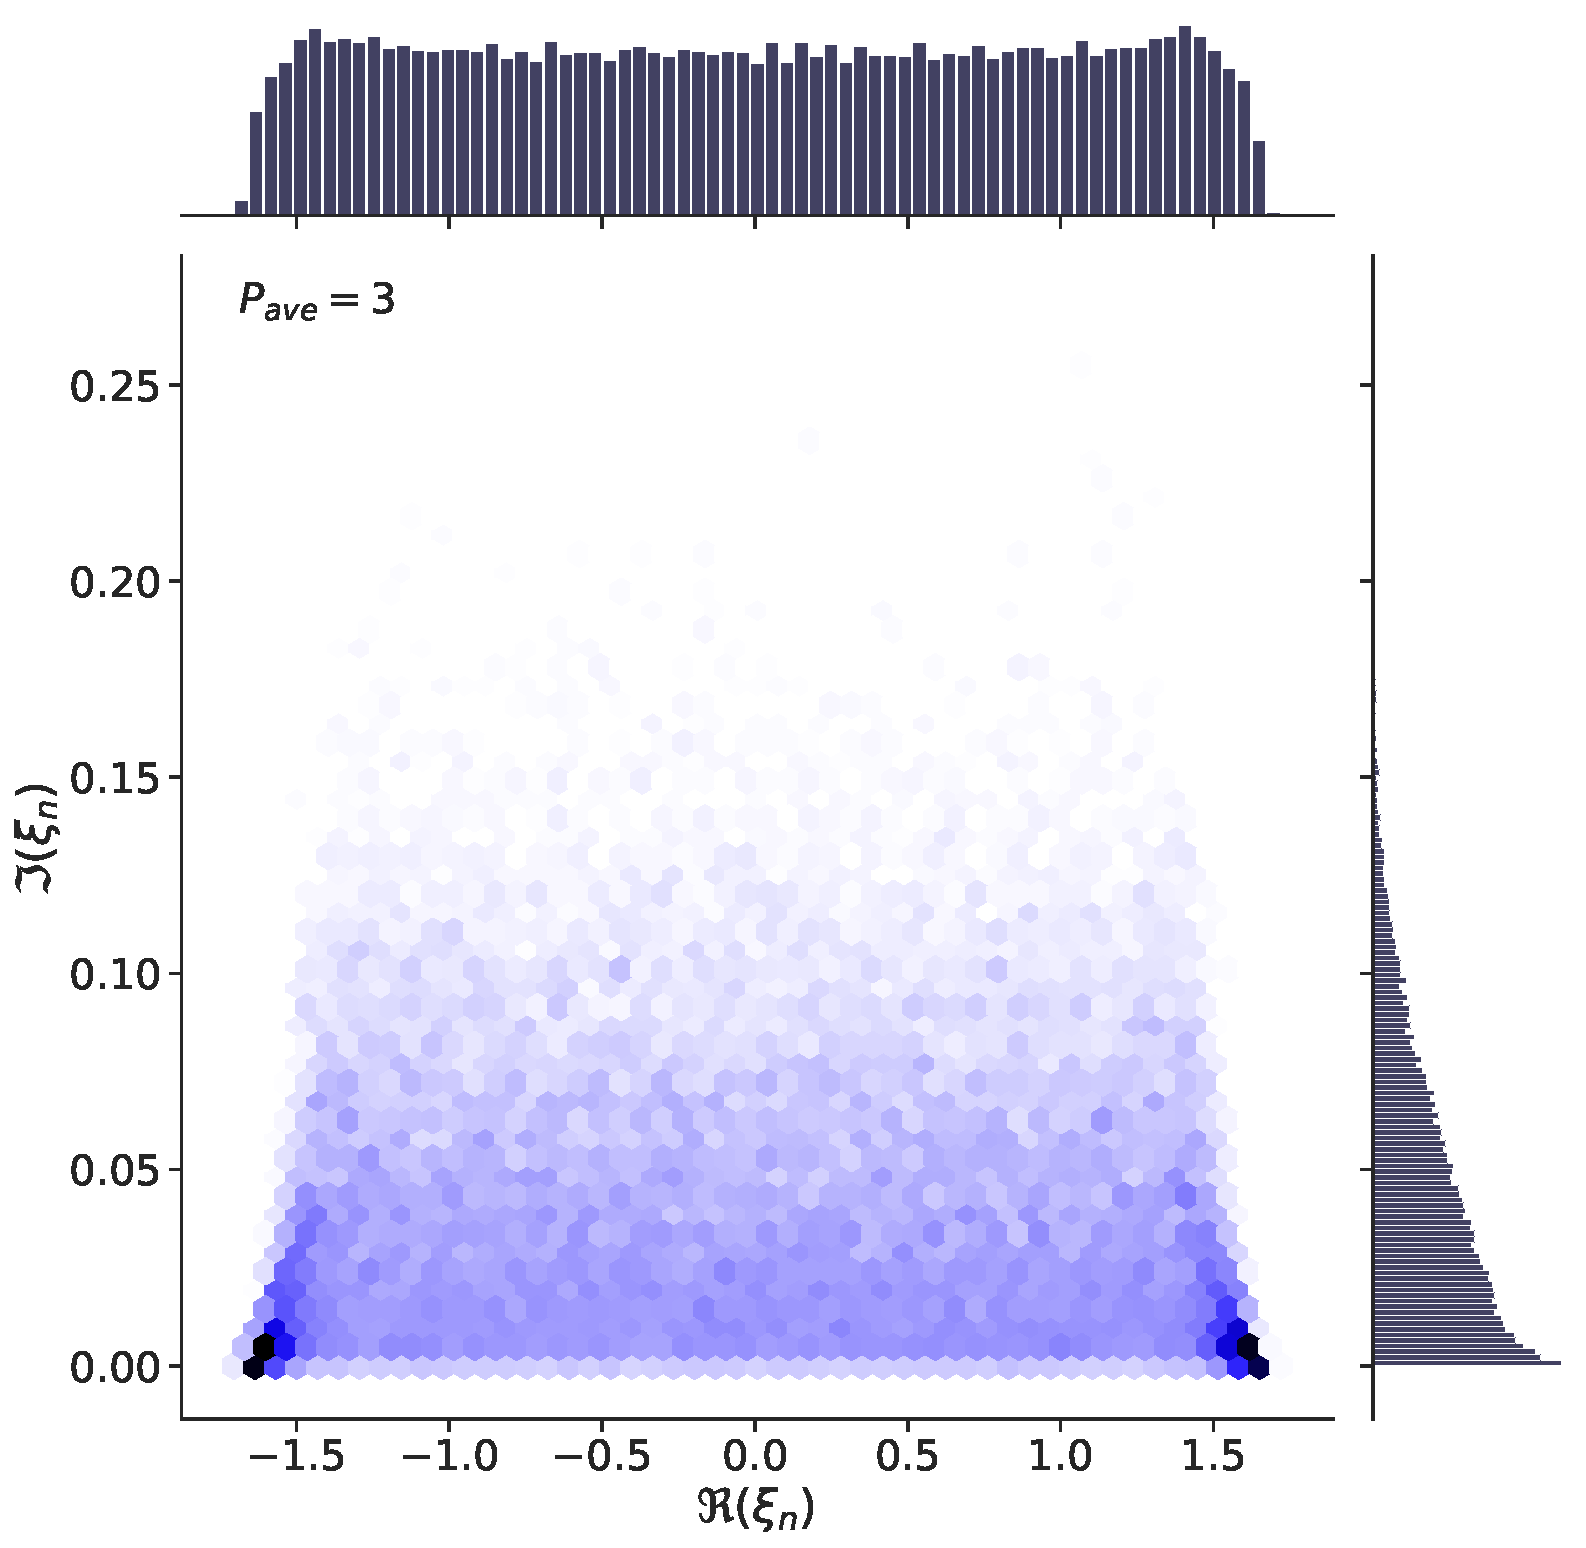
\includegraphics[width=1\linewidth]{images/soliton/wdm_trans/discrete_spectrum_distribution_pavedbm_3.pdf} \\
    }
    \end{minipage}
    \hfill
    \begin{minipage}[h]{0.49\linewidth}
    \center{
        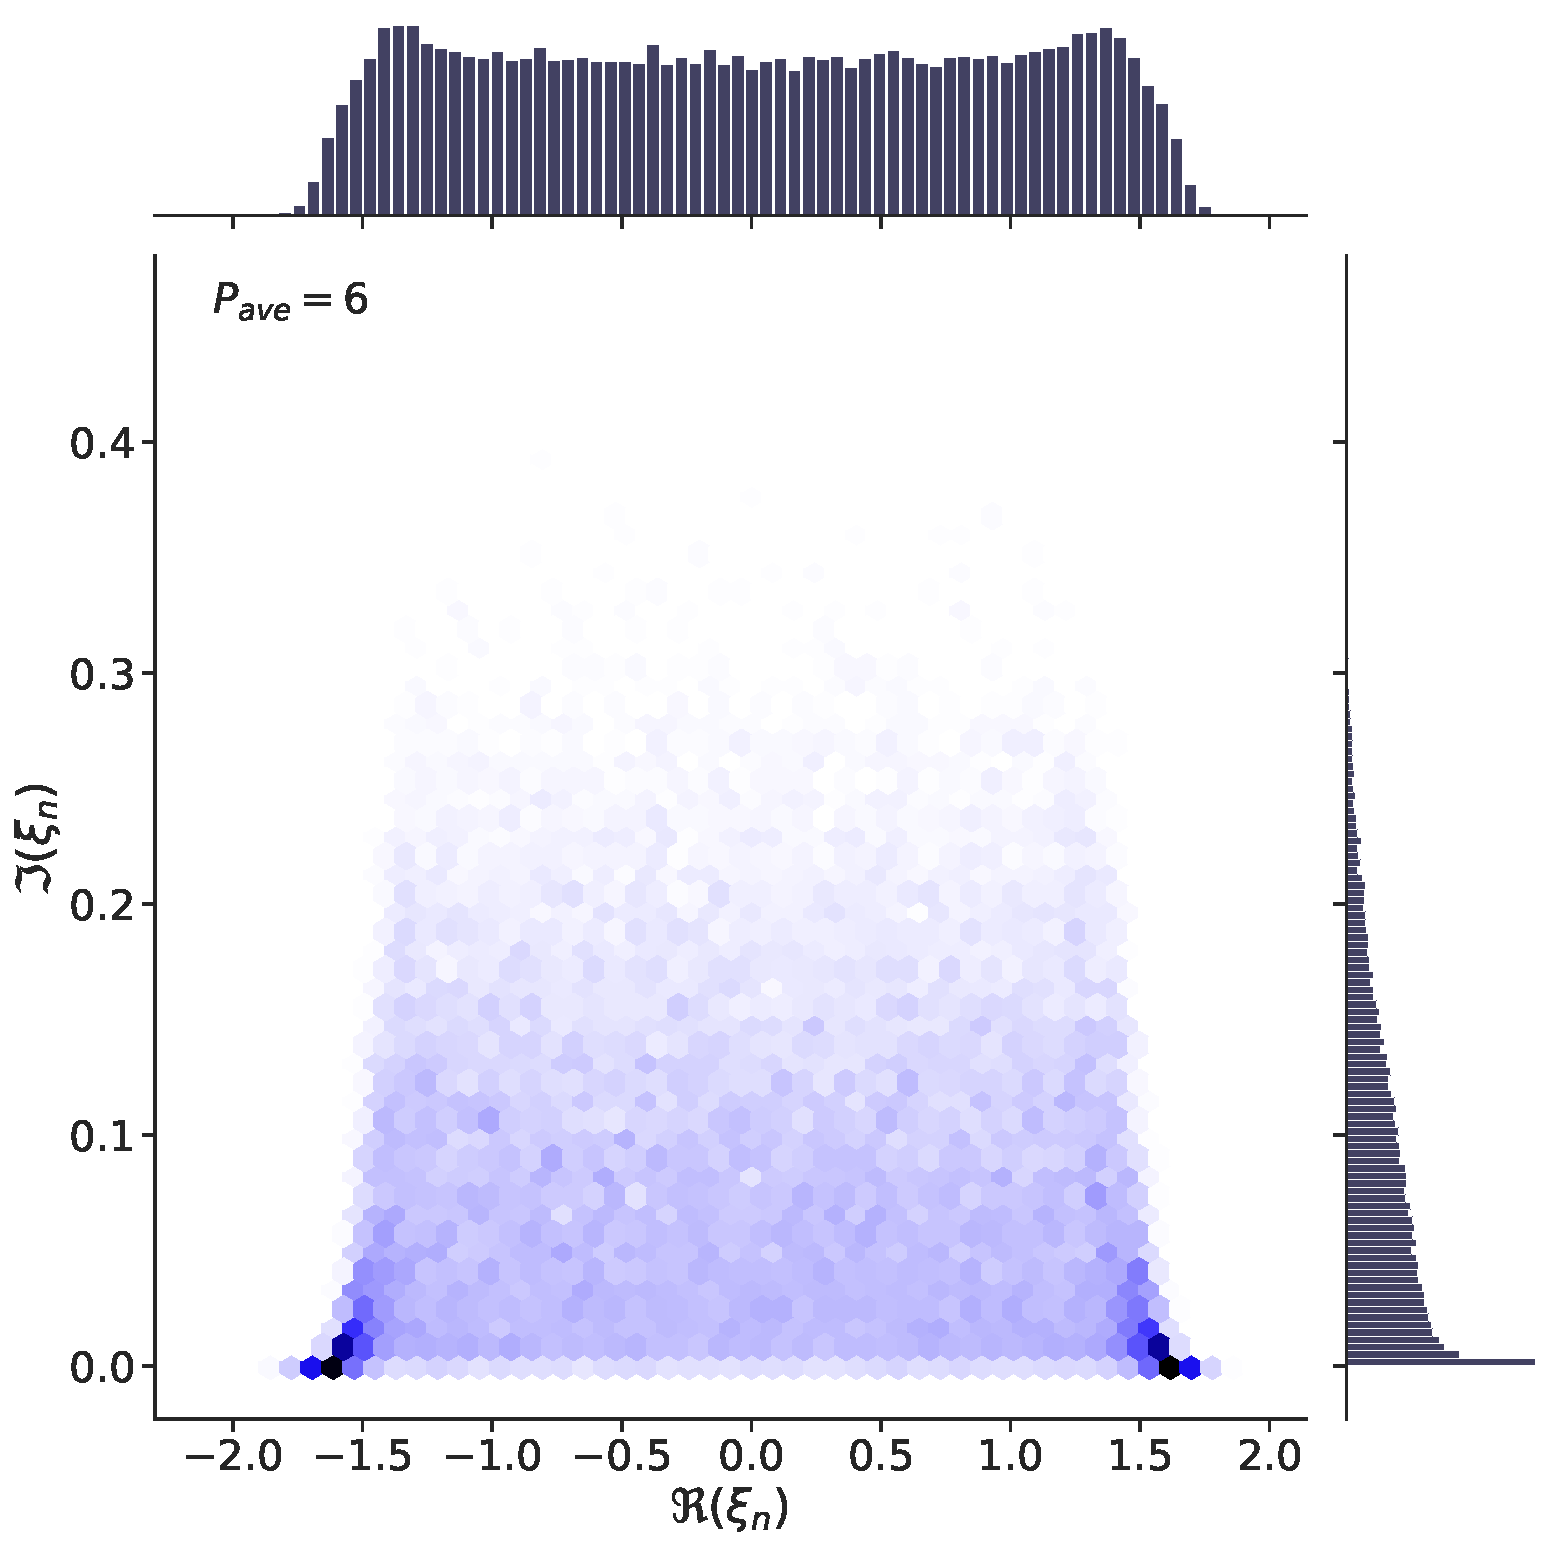
\includegraphics[width=1\linewidth]{images/soliton/wdm_trans/discrete_spectrum_distribution_pavedbm_6.pdf} \\
    }
    \end{minipage}
    \caption{Distribution of discrete eigenvalues in the NF spectrum across the complex plane at varying signal power levels, beginning at -15 dBm in the upper left and concluding at 6 dBm in the lower right panels.}
    \label{fig:wdm_trans_sol_full_distr}
\end{figure}